\documentclass[14pt, dvipsnames]{extarticle}
\usepackage[left=2cm, top=2cm, right=2cm, bottom=20mm]{geometry} 
\usepackage[utf8x]{inputenc} % Включаем поддержку UTF8
\usepackage[russian]{babel}  % Включаем пакет для поддержки русского языка
\usepackage{ucs}
\usepackage{tikzsymbols}
 \usepackage{fontawesome}
 \usepackage{simpsons}
 \usepackage{xcolor}
 
\usepackage{wrapfig}
  
\usepackage{amsthm, amsmath, amssymb} % Mathematical typesetting
\usepackage{hyperref} % For hyperlinks in the PDF

\usepackage{esint}
 
\newtheorem{theorem}{Теорема}
\newtheorem{statement}{Утверждение}
\newtheorem*{lemma}{Лемма}
\newtheorem*{proposition}{Предложение}
\newtheorem*{conseq}{Следствие}
\newtheorem{question}{Вопрос}


\theoremstyle{definition}
\newtheorem{defi}{Определение}
\newtheorem{property}{Свойство}
\newtheorem{problem}{Задача}
\newtheorem{exercise}{Упражнение}
\newtheorem{example}{Пример}

\theoremstyle{remark}
\newtheorem*{comment}{\sc Замечание}

\usepackage{enumerate}






\usepackage{fancybox,fancyhdr}
\usepackage{lipsum}
\fancyhead[R]{}
\fancyhead[C]{\sc\leftmark}
\fancyhead[L]{}
%\renewcommand{\headrulewidth}{0.5pt}
%\renewcommand{\footrulewidth}{0.5pt}
\fancyfoot[C]{\hrulefill\protect\circled{\thepage}\hrulefill}

\usepackage{tikz}
\newcommand*\circled[1]{\tikz[baseline]{\node[shape=circle,draw,inner sep=2pt] (char) {#1};}}






\usepackage{asymptote}

\usepackage[all]{xy}

\DeclareMathOperator{\Tor}{\mathrm{Tor}\!}
\DeclareMathOperator{\End}{\mathrm{End}\,}
\DeclareMathOperator{\Sq}{\mathrm{Sq}}
\DeclareMathOperator{\cp}{\smallsmile}
\DeclareMathOperator{\Hom}{\mathrm{Hom}}
\DeclareMathOperator{\Sp}{\mathrm{Sp}}
\DeclareMathOperator{\Z2}{\mathbb{Z}_2}
\DeclareMathOperator{\CP}{\mathbb{C}P}
\DeclareMathOperator{\CC}{\mathbb{C}\!}
\DeclareMathOperator{\Th}{\mathrm{Th}}

\renewcommand{\phi}{\varphi}

\usepackage{textcomp}

\usepackage{mathabx}

%Некий костыль с двух сторон от декларации пакета bm
\let\saveboldsymbol\boldsymbol
\usepackage{bm}
\let\boldsymbol\saveboldsymbol

\usepackage{mathrsfs} 

\usepackage{indentfirst}

\newcommand{\factor}[2]{{\raisebox{.2em}{$#1$}\left/\raisebox{-.2em}{$#2$}\right.}}

\usepackage{titlesec}



\begin{document}


Покажем, что модификация Маундера конструкции Кана-Тёрстона может давать для двумерного симплекса (треугольника) двумерный комплекс с нетривиальной фундаментальной группой. Построение будем вести последовательно.

Сначала мы имели нульмерный остов, состоящий из 3 вершин $L = \{0, 1,  2\}$. В этом случае конус $CL = \{ [3, 0], [3, 1], [3, 2] \}$. Конструкция Кана-Тёрстона $TL$ совпадёт с $L$ и пространство $UL$ совпадёт с $CL$. Отображение пар $t: (UL, TL) \to (CL, L)$ будем считать тождественным.

{\bf Шаг 1.} Приклеим 1-симплекс $\sigma = [0, 1]$ к комплексу $L$ и получим комплекс $K$. Тогда $C\partial \sigma$ будет <<рогом>> $[3, 0]\cup [3, 1]$, и $t^{-1}(C\partial \sigma) = [3, 0]\cup [3, 1]$, и $t^{-1}(\partial\sigma) = [0]\cup [1]$. Значит, $TK = TL\sqcup_{t^{-1}(\partial\sigma)} t^{-1}(C\partial\sigma) = [0, 1]\cup [2]$ --- это объединение отрезка и точки, причём при отображении $t$ вершина конуса $[3]$ отображается в середину отрезка $[0, 1]$. 

\begin{center}
\includegraphics[scale=0.5]{pict1}
\end{center}


Пространство $X = t^{-1}(C\partial\sigma)\sqcup_{t^{-1}(\partial\sigma)} t^{-1}(C\partial\sigma) = [3, 0]\cup [3,1] \cup [3', 0] \cup [3', 1]$ --- это окружность $K(\mathbb{Z}, 1)$. 

\begin{center}
\includegraphics[scale=0.5]{pict2}
\end{center}


Далее, мы должны приклеить к объединение $UL\cup TK$ к пространству $X$. В результате получится: 


\begin{center}
\includegraphics[scale=0.5]{pict3}
\end{center}


Теперь нужно приклеить к пространству $(UL\cup TK)\cup X$ цилиндр отображения $K(\mathbb{Z}, 1)\to K(\mathrm{Hig}_4), 1$, и мы получим пространство $UK$. Обозначим для удобства дальнейшего изложения получившееся образования за $A:=UK$. 


\begin{center}
\includegraphics[scale=0.5]{pict4}
\end{center}





{\bf Шаг 2.} Переобозначим полученную комплексов через $(UL, TL)$ и будем приклеивать следующий 1-симплекс $[1, 2]$.

Пока мы имеем такие данные:   

\begin{center}
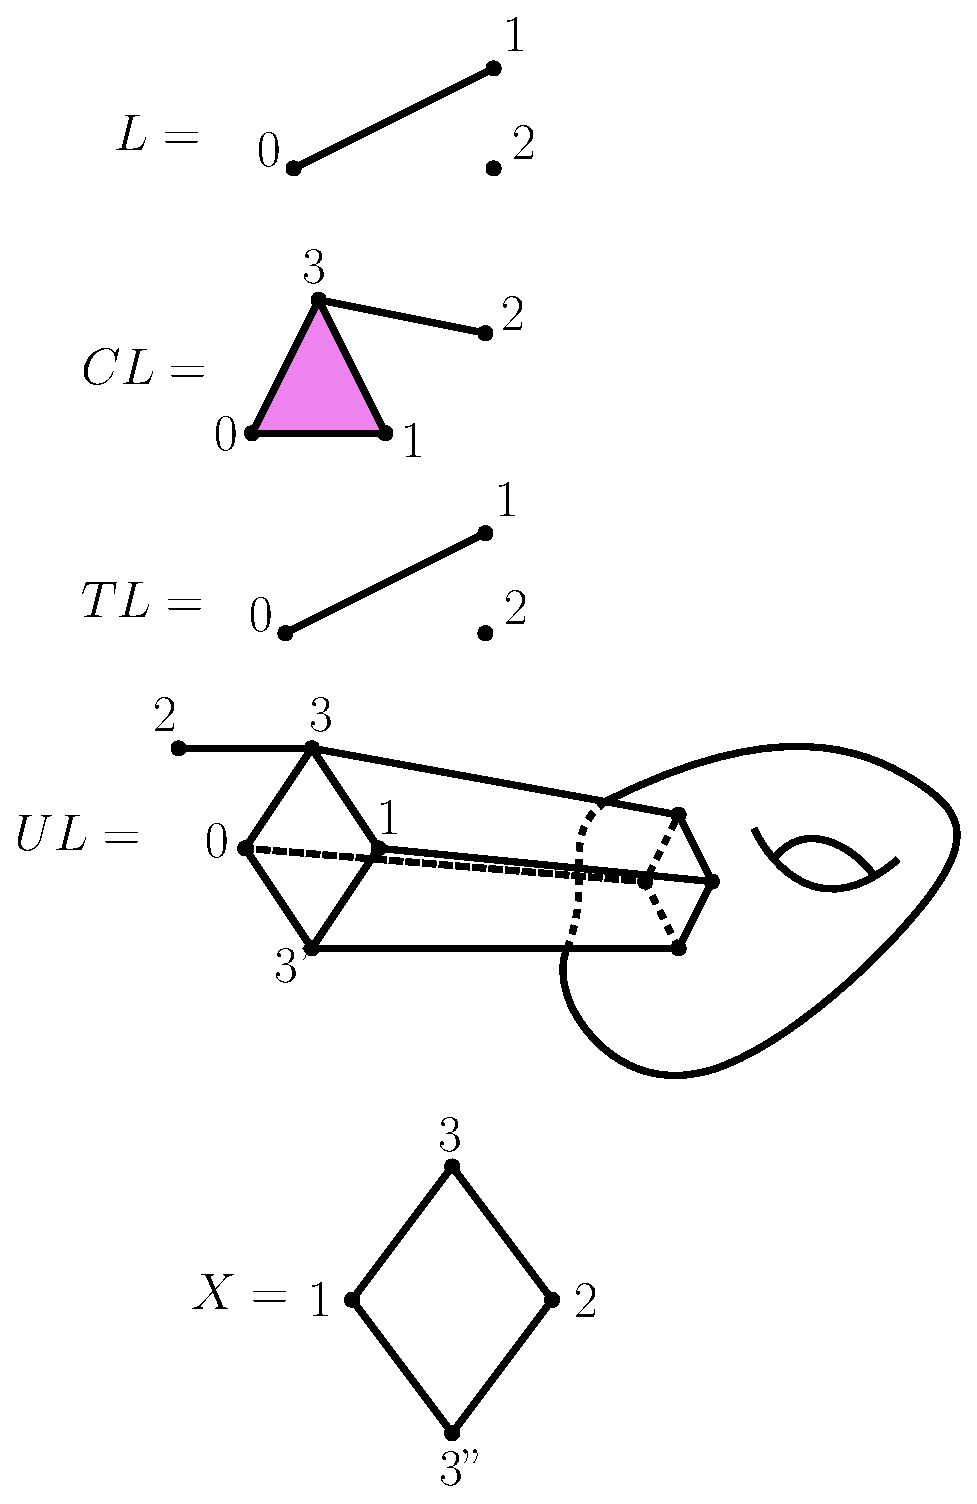
\includegraphics[scale=0.4]{pict5}
\end{center}
 

В результате, в качестве пространства $UK$ будет выступать пространство с двумя копиями $A$, причём вторая копия $A$ будет подклеиваться к <<рогу>> $[3,2]\cup [3, 1]$.


{\bf Шаг 3.} Приклеим третье ребро $[0, 2]$. В результате подклеится ещё одна копия пространства типа $A$ с прошлого шага, но уже к рогу $[3, 2]\cup [3, 0]$ --- в случае построения нового $UK$. Пространство Кана-Тёрстона же будет по-прежнему совпадать с исходным пространством, то есть будет границей треугольника.



{\bf Шаг 4.} Подклейка двумерной клетки к границе треугольника. В итоговой конструкции $T\Delta^2$ будет иметься уже три образования типа $A$, склеенных вдоль рогов трёх рогов с общей вершиной $[3]$ и остальными вершинами $[0], [1], [2]$. Приведём здесь схему расположения <<рогов>>:


\begin{center}
\includegraphics[scale=0.5]{pict7}
\end{center}
 
 
Таким образом, $T\Delta^2$ получено не является стягиваемым пространством по теореме ван Кампена, поэтому $T\Delta^2$ не гомеоморфно $\Delta^2$.







































\end{document}